\section{Auswertung}
\subsection{Einzelspalt ($0{,}075\,\symup{mm}$)}

Zunächst wird die Beugungsfigur eines Einfach-Spaltes ausgemessen, dessen Breite von $b_{\text{t1}} = 0{,}075\,\symup{mm}$ vom Hersteller angegeben ist und als Theoriewert dient.
In Tabelle \ref{tab:1} sind die eingestellten Schrittweiten in $\symup{mm}$ sowie die jeweils gemessenen Stromstärken in $\mu m$ zu finden. Die Einstellungen der Photodiode auf dem Messreiter
wurden dabei um $+0{,}94\,\symup{mm}$ verschoben, sodass sich die maximale Lichtintensität bei $0\,\symup{mm}$ befindet. Der vor dem Versuch gemessene Dunkelstrom von 
\begin{equation*}
I_{\text{du}} = 4{,}3\,\symup{nA}
\end{equation*} 
wird für den Plot von allen Stromstärken $I$ abgezogen. Dieser ergibt sich durch Auftragen der Stromstärken $I-I_{\text{du}}$ gegen die Schrittweiten $x$ und ist in Abbildung \ref{fig:es1} zu finden. 

\begin{table}[h!tbp]
\centering
\caption{Messwerte zur Untersuchung des Einzelspaltes mit $0{,}075\,\symup{mm}$.}
\label{tab:1}
\begin{tabular}{S[table-format=2.2, table-auto-round] S[table-format=1.5, table-auto-round] S[table-format=2.2, table-auto-round] S[table-format=1.4, table-auto-round] }
\toprule
{x/$10^{-3}\,\symup{m}$} & {I/$10^{-6}\,\symup{A}$} & {x/$10^{-3}\,\symup{m}$} & {I/$10^{-6}\,\symup{A}$}  \\
\midrule
-20.0 & 0.0087  & 0.94 & 0.31\\
-19.0 & 0.0108  & 1.88 & 0.28\\
-18.0 & 0.0126  & 2.88 & 0.22\\
-17.5 & 0.01305 & 3.88 & 0.162\\	   
-17.0 & 0.01275 & 4.88 & 0.099\\
-16.0 & 0.0111  & 5.88 & 0.048\\
-15.0 & 0.0087  & 6.88 & 0.021\\
-14.0 & 0.0075  & 7.88 & 0.0099\\
-13.0 & 0.009   & 8.88 & 0.018\\
-12.0 & 0.0132  & 10.88 & 0.0138\\
-11.0 & 0.017   & 11.88 & 0.0156\\
-10.0 & 0.022   & 12.88 & 0.0106\\
-9.18  & 0.0224  & 13.88 & 0.0066\\
-9.0  & 0.02    & 14.88 & 0.0046\\ 
-8.0  & 0.014   & 15.88 & 0.0056\\
-7.0  & 0.01    & 16.88 & 0.0072\\
-6.0  & 0.0385  & 17.88 & 0.0079\\
-5.0  & 0.078   & 18.01 & 0.008\\
-4.0  & 0.141   & 18.88 & 0.0073\\
-3.0  & 0.19    & 19.88 & 0.006\\
-2.0  & 0.265   & 20.88 & 0.0045\\
-1.0  & 0.31    & 21.88 & 0.0036\\
 0.0  & 0.35    &       & \\
\bottomrule
\end{tabular}
\end{table}


\begin{figure}[h!tbp]
	\centering
	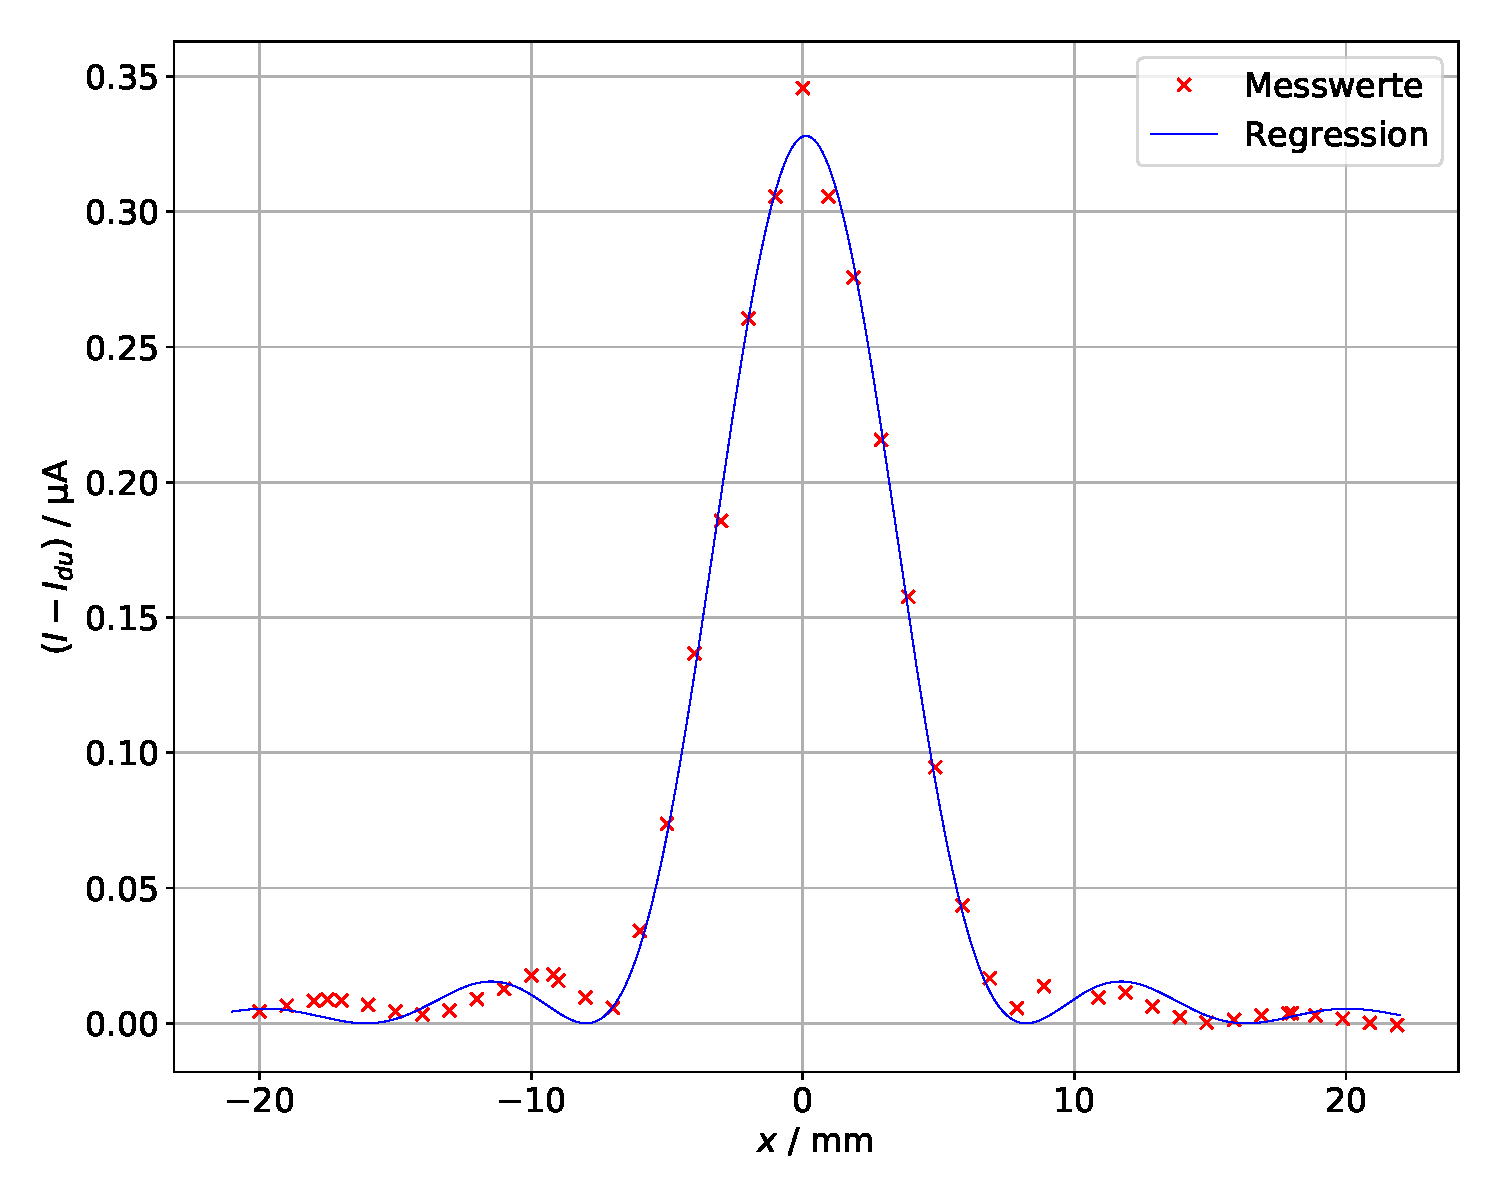
\includegraphics[width=1\linewidth]{einzel75.pdf}
	\caption{Stromstärke $I-I_{\text{du}}$ als Funktion der Schrittweite $x$, sowie nichtlineare Regression für den Einfach-Spalt mit $0{,}075\,\symup{mm}$.}
	\label{fig:es1}
\end{figure}

Mithilfe des Python-Moduls matplotlib wird mit Gleichung \ref{eq:eq5} eine nichtlineare Ausgleichsrechnung durch die Messwerte vorgenommen, wie in Abildung \ref{fig:es1} zu sehen ist.
Diese Ausgleichsrechnung liefert einen experimentellen Wert der Spaltbreite $b_{\text{es,1}}$:

\begin{equation*}
b_{\text{es,1}} = (0{,}0784\pm 0{,}0008)\,\symup{mm}.
\end{equation*}





\newpage
\subsection{Einzelspalt ($0{,}15\,\symup{mm}$)}
Nun wird ein Einzelspalt der Breite $b_{\text{t2}} = 0{,}15\,\symup{mm}$ untersucht. Tabelle \ref{tab:2} enthält die aufgenommen Messdaten. Zu den Werten von $x$ werden hier $1\,\symup{mm}$ addiert.
Für den Plot wird wieder der Dunkelstrom $I_{\text{du}}$ von den gemessenen Strömen abgezogen.

\begin{table}[h!tbp]
\centering
\caption{Messwerte zur Untersuchung des Einzelspaltes mit $0{,}15\,\symup{mm}$.}
\label{tab:2}
\begin{tabular}{S[table-format=2.2, table-auto-round] S[table-format=1.4, table-auto-round] S[table-format=2.1, table-auto-round] S[table-format=1.4, table-auto-round] }
\toprule
{x/$10^{-3}\,\symup{m}$} & {I/$10^{-6}\,\symup{A}$} & {x/$10^{-3}\,\symup{m}$} & {I/$10^{-6}\,\symup{A}$}  \\
\midrule
-11.5 & 0.022 & 2.0 & 0.34 \\
-11.1 & 0.027 & 2.5 & 0.192 \\
-10.6 & 0.03 & 2.8 & 0.108 \\
-9.9 & 0.026 & 3.0 & 0.069 \\
-9.4 & 0.0198 & 3.3 & 0.36 \\
-9.2 & 0.0156 & 3.5 & 0.02 \\
-8.9 & 0.0114 & 3.8 & 0.0138 \\
-8.5 & 0.0102 & 4.0 & 0.015 \\
-8.3 & 0.012 & 4.2 & 0.0204 \\
-8.0 & 0.016 & 4.4 & 0.0288 \\
-7.8 & 0.023 & 4.6 & 0.036 \\
-7.5 & 0.034 & 4.7 & 0.04 \\
-7.3 & 0.044 & 4.8 & 0.046 \\
-6.9 & 0.064 & 4.9 & 0.05 \\
-6.6 & 0.076 & 5.2 & 0.06 \\ 
-6.07 & 0.087 & 5.5 & 0.066 \\
-5.5 & 0.076 & 6.0 & 0.062 \\
-5.3 & 0.068 & 6.4 & 0.052 \\
-5.0 & 0.051  & 6.6 & 0.045 \\
-4.8 & 0.041 & 6.9 & 0.033 \\
-4.6 & 0.031 & 7.6 & 0.0153 \\
-4.4 & 0.036 & 7.9 & 0.0105 \\
-4.0 & 0.04 & 8.1 & 0.009 \\
-3.8 & 0.058 & 8.8 & 0.0114 \\
-3.5 & 0.09 & 9.3 & 0.0156 \\
-3.3 & 0.132 & 9.84 & 0.0174 \\
-3.0 & 0.216 & 10.5 & 0.0147 \\
-2.0 & 0.54 & 10.8 & 0.012 \\
-1.0 & 0.93 & 11.1 & 0.009 \\
0.0  & 1.05 & 11.3  & 0.0078 \\

\bottomrule
\end{tabular}
\end{table}


\begin{figure}[h!tbp]
	\centering
	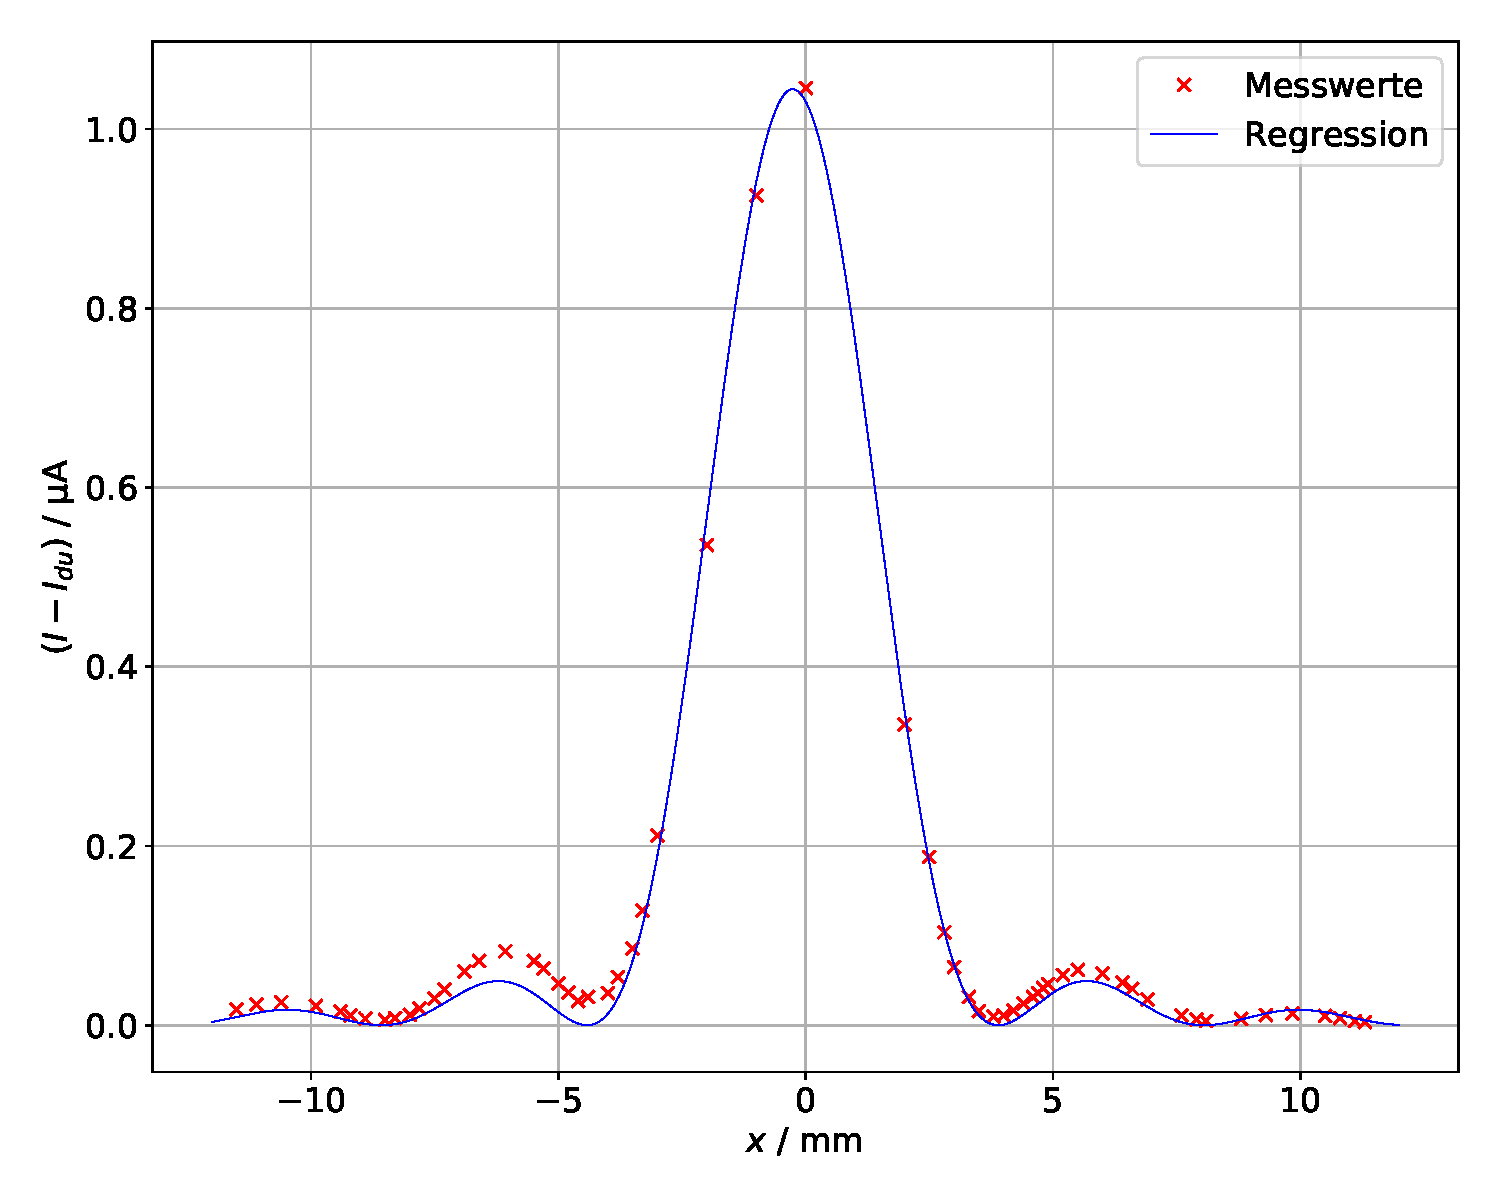
\includegraphics[width=1\linewidth]{es2.pdf}
	\caption{Stromstärke $I-I_{\text{du}}$ als Funktion der Schrittweite $x$, sowie nichtlineare Regression für den Einfach-Spalt mit $0{,}15\,\symup{mm}$.}
	\label{fig:es2}
\end{figure}

Die aufgetragenen Messdaten, sowie die Ausgleichsrechnung, die analog zum ersten Versuchsteil erfolgt, sind in Abbildung \ref{fig:es2} zu sehen.
Die Regression ergibt eine Spaltbreite $b_{\text{es,2}}$ von:

\begin{equation*}
b_{\text{es,2}} = (0{,}15279\pm 0{,}00116)\,\symup{mm}.
\end{equation*}



\subsection{Doppelspalt}

Zuletzt wird ein Doppelspalt untersucht, dessen Spaltbreite $b_{\text{t3}} = 0{,}15\,\symup{mm}$ beträgt, während der Abstand zwischen den beiden Spalten $g = 0{,}25\,\symup{mm}$ ist.
Alle Messwerte sind in den Tabellen \ref{tab:3} und \ref{tab:4} zu finden.
Auf die Einstellungen $x$ werden in diesem Fall $0{,}8\,\symup{mm}$ addiert und der Dunkelstrom abermals abgezogen. 
Die Regression erfolgt wiederum mit Python, wobei nun Gleichung \ref{eq:dsg} verwendet wird. Zudem wird analog zu den vorherigen Versuchteilen die Beugungsfigur eines Einfach-Spaltes hinzugefügt, wie in Abbildung \ref{fig:ds} zu sehen ist.


\begin{table}[h!tbp]
\centering
\caption{Messwerte zur Untersuchung des Doppelspaltes.}
\label{tab:3}
\begin{tabular}{S[table-format=2.1, table-auto-round] S[table-format=1.4, table-auto-round] S[table-format=2.1, table-auto-round] S[table-format=1.3, table-auto-round] S[table-format=2.1, table-auto-round] S[table-format=1.3, table-auto-round] S[table-format=2.1, table-auto-round] S[table-format=1.3, table-auto-round] }
\toprule
{x/$10^{-3}\,\symup{m}$} & {I/$10^{-6}\,\symup{A}$} & {x/$10^{-3}\,\symup{m}$} & {I/$10^{-6}\,\symup{A}$} & {x/$10^{-3}\,\symup{m}$} & {I/$10^{-6}\,\symup{A}$} & {x/$10^{-3}\,\symup{m}$} & {I/$10^{-6}\,\symup{A}$}   \\
\midrule
-14.7 & 0.0087 & -6.4 & 0.039 & -0.4 & 2.9 & 2.2 & 0.108  \\
-14.3 & 0.0102 & -6.1 & 0.057 & -0.3 & 3.3 & 2.3 & 0.108  \\ 
-4.2 & 0.0111 & -5.6 & 0.138 & 0.0 & 3.8 & 2.4 & 0.102 \\ 
-13.6 & 0.014 & -5.4 & 0.168 & 0.3 & 3.3 & 2.5 & 0.093  \\
-13.3 & 0.02 & -5.2 & 0.18 & 0.5 & 2.6 & 2.6 & 0.084 \\
-12.8 & 0.03 & -4.9 & 0.156 & 0.6 & 2.1 & 2.7 & 0.0774 \\
-12.4 & 0.027 & -4.7 & 0.12 & 0.8 & 1.5 & 2.8 & 0.0624  \\
-11.6 & 0.014 & -3.9 & 0.03 & 0.9 & 1.08 & 3.0 & 0.047  \\
-11.2 & 0.017 & -3.8 & 0.033 & 1.0 & 0.081 & 3.2 & 0.029 \\
-10.8 & 0.03 & -3.7 & 0.042 & 1.1 & 0.06 & 3.3 & 0.022  \\
-10.3 & 0.064 & -3.6 & 0.054 & 1.2 & 0.052 & 3.4 & 0.016  \\
-9.94 & 0.074 & -3.4 & 1.102 & 1.3 & 0.044 & 3.6 & 0.102  \\
-9.8 & 0.072 & -3.2 & 0.17 & 1.4 & 0.043 & 3.8 & 0.063  \\
-9.6 & 0.062 & -2.9 & 0.41 & 1.5 & 0.048 & 4.0 & 0.051  \\
-9.4 & 0.047 & -2.5 & 0.75 & 1.6 & 0.06 & 4.3 & 0.066  \\
-8.9 & 0.018 & -2.0 & 0.93 & 1.7 & 0.072 & 4.5 & 0.093  \\
-8.5 & 0.016 & -1.8 & 0.77 & 1.8 & 0.086 & 4.6 & 0.114  \\
-8.0 & 0.02 & -1.3 & 0.48 & 1.9 & 0.09 & 4.7 & 0.132 \\
-7.5 & 0.03 & -1.0 & 0.78 & 2.0 & 0.102 & 4.8 & 0.15  \\
-6.8 & 0.042 & -0.8 & 1.44 & 2.1 & 0.105 & 4.9 & 0.162 \\



\bottomrule
\end{tabular}
\end{table}

\begin{table}[h!tbp]
\centering
\caption{Messwerte zur Untersuchung des Doppelspaltes.}
\label{tab:4}
\begin{tabular}{S[table-format=1.2, table-auto-round] S[table-format=1.4, table-auto-round] S[table-format=2.1, table-auto-round] S[table-format=1.4, table-auto-round] S[table-format=2.1, table-auto-round] S[table-format=1.5, table-auto-round]}
\toprule
{Messung} & {Zählrate} & {Messung} & {Zählrate} & {Zählrate} & {Zählrate}   \\
\midrule
4.9 & 0.162 & 8.2 & 0.024 & 14.8 & 0.0192\\
5.0 & 0.171 & 8.4 & 0.053 & 15.1 & 0.01914\\ 
5.2 & 0.1746 & 9.1 & 0.068 & 15.6 & 0.0141\\ 
5.3 & 0.168 & 9.5 & 0.071 & 16.0 & 0.009\\
5.4 & 0.153 & 9.7 & 0.074 & &\\
5.5 & 0.138 & 9.8 & 0.072 & &\\
5.6 & 0.1194 & 9.9 & 0.067 & &\\
5.8 & 0.075 & 10.1 & 0.038 & &\\
6.0 & 0.042 & 10.2 & 0.0201 & &\\
6.2 & 0.028 & 10.6 & 0.0135 & &\\
6.4 & 0.021 & 10.9 & 0.0114 & &\\
6.6 & 0.0279 & 11.1 & 0.0123 & &\\
6.7 & 0.033 & 11.3 & 0.024 & &\\
6.8 & 0.039 & 11.5 & 0.026 & &\\
6.9 & 0.042 & 12.0 & 0.03 & &\\
7.1 & 0.049 & 12.2 & 0.0108 & &\\
7.18 & 0.05 & 12.7 & 0.009 & &\\
7.5 & 0.045 & 13.6 & 0.0075 & &\\
7.7 & 0.039 & 14.4 & 0.0138 & &\\
7.8 & 0.038 & 14.6 & 0.0174 & &\\



\bottomrule
\end{tabular}
\end{table}


\begin{figure}[h!tbp]
	\centering
	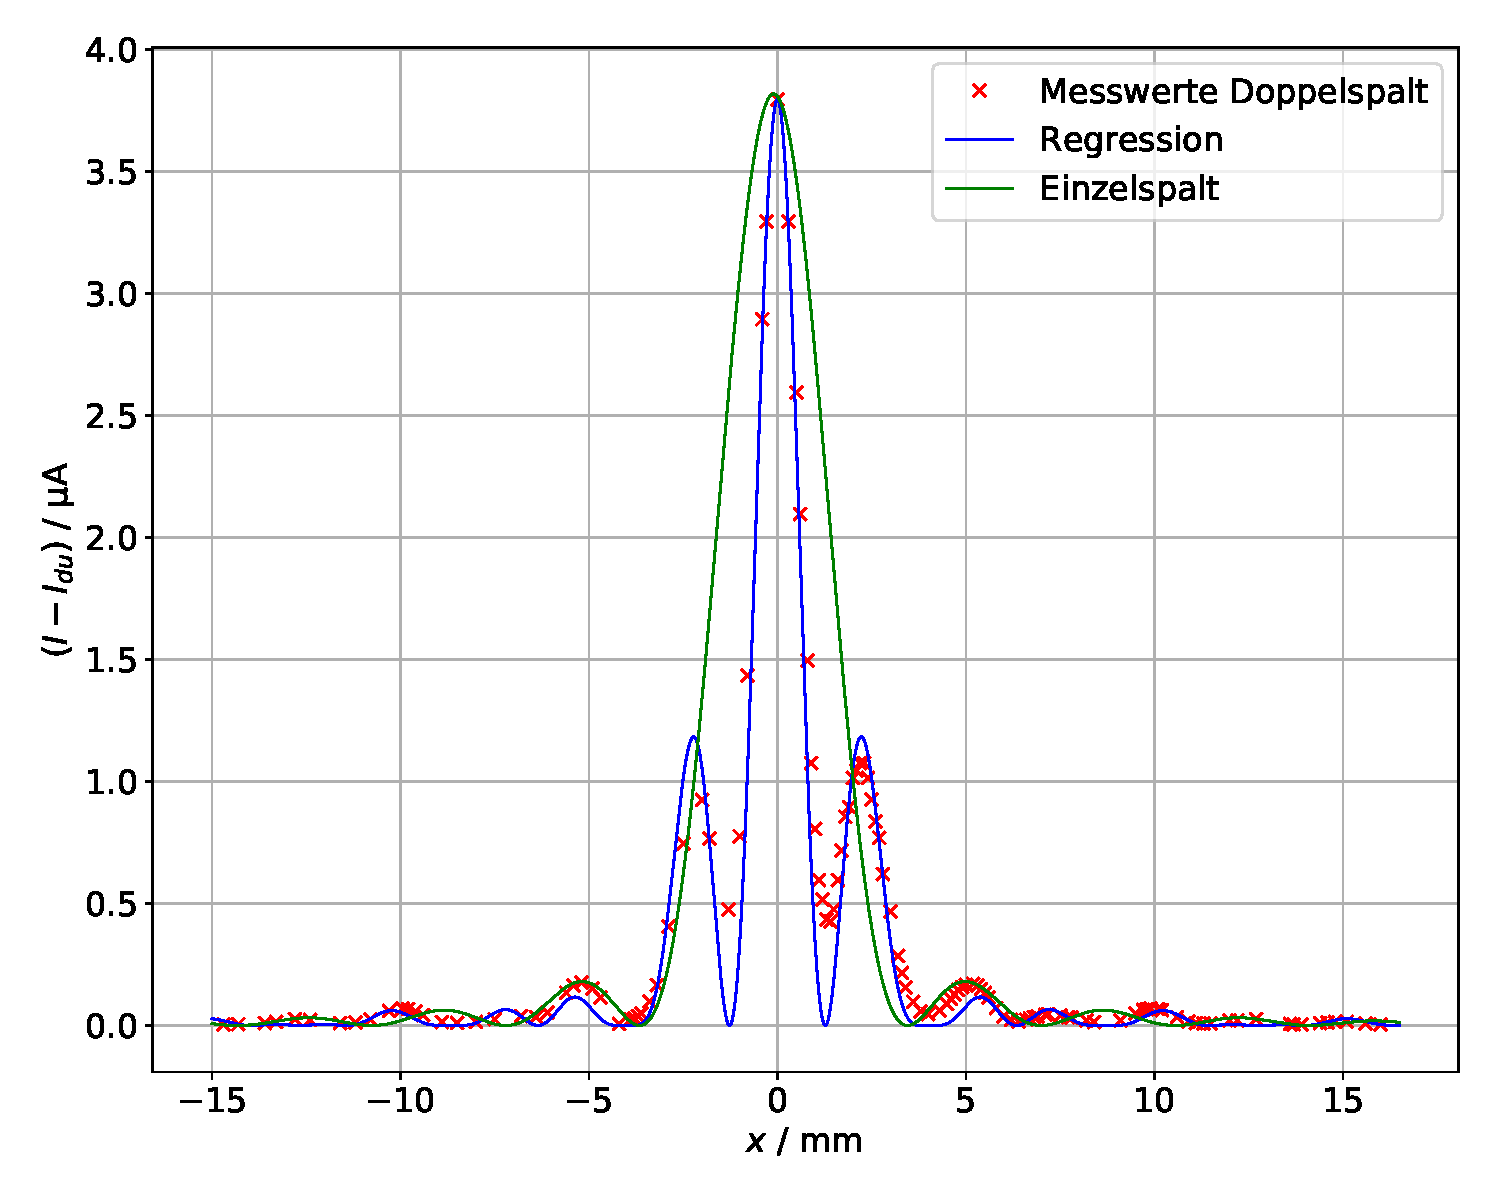
\includegraphics[width=1\linewidth]{ds.pdf}
	\caption{Stromstärke $I-I_{\text{du}}$ als Funktion der Schrittweite $x$, sowie nichtlineare Regression für den Doppelspalt.}
	\label{fig:ds}
\end{figure}